\documentclass[../main.tex]{subfiles}
\begin{document}
	
	\section{Lista 3}
		\subsection{Parte 1 (computacional)}
		\begin{exercicio}{1}
			Resolver em ambiente computacional o exercício 1 da seção 8.3 (pag 276) do livo do Apostol de Cálculo 2. Explore os recursos de plot da ferramenta computacional escolhida por você para exibir as curvas e superfícies de nível.
		\end{exercicio}
		
		\begin{solucao}
			Nos itens a), b) e c), temos
			\begin{enumerate}[label=\alph*)]
				\item $f(x,y)=x^2+y^2$
				\item $f(x,y)=e^{xy}$
				\item $f(x,y)=\cos(x+y)$
			\end{enumerate}
			
			
			Sendo todos campos escalares do tipo $f:S\subset \mathbb{R}^2\rightarrow \mathbb{R}$, podemos representar as curvas de nível no plano, por meio da função "contour plot", ou na superfície, dada pelo conjunto de pontos $(x,y,f(x,y))$. Nas figuras 1 a 6 temos as imagens plotadas.
			
			\begin{lstlisting}[style=python_estiloso, caption={estrutura do código da questão 1, itens a), b), c)}]
				#Definindo as variaveis
				var("x y z")
				
				# 1. Grafico da superficie
				superficie_plot = plot3d('equacao', (x, -3, 3), (y, -3, 3), color='gray')
				
				# 2. Representando as curvas de nivel na superficie
				curva_nivel_3d1 = implicit_plot3d('equacao' == valor1,
				(x, -5, 5), (y, -5, 5), (z, -0.1, 0.1), color='purple', thickness=10)
				curva_nivel_3d2 = implicit_plot3d('equacao' == valor2,
				(x, -5, 5), (y, -5, 5), (z, 0.9, 1.1), color='red', thickness=10)
				curva_nivel_3d3 = implicit_plot3d('equacao' == valor3,
				(x, -5, 5), (y, -5, 5), (z, 3.9, 4.1), color='yellow', thickness=10)
				curva_nivel_3d4 = implicit_plot3d('equacao' == valor4,
				(x, -5, 5), (y, -5, 5), (z, 8.9, 9.1), color='green', thickness=10)
				
				# 3. Combinando os graficos
				resultado_final = superficie_plot + curva_nivel_3d1 + curva_nivel_3d2 + 
				curva_nivel_3d3 + curva_nivel_3d4
				
				# Exibindo o grafico combinado
				resultado_final.show(aspect_ratio=[1,1,1], 
				title='Superficie e Curvas de Nivel no 3D')
				contour_plot((x^2 + y^2), (x, -2, 2), (y, -2, 2), 
				contours=20, cmap='ocean', title='Curvas de Nivel de equacao')
			\end{lstlisting}
			
			\begin{center}
				% Primeira imagem
				\begin{minipage}{0.45\textwidth}
					\centering
					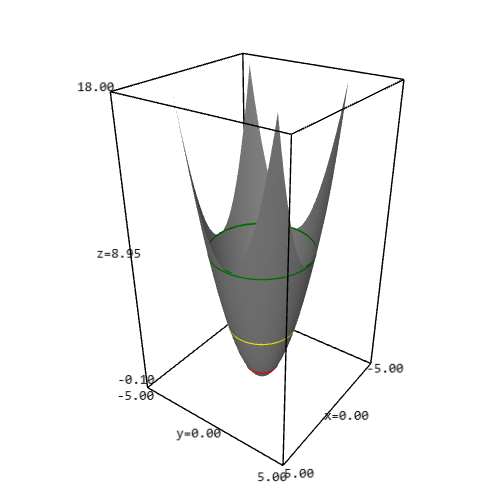
\includegraphics[width=\textwidth]{imagens/lista03/picture_lista03_q01_item01.png}
					\captionof{figure}{questão 1, item a), superfície}
				\end{minipage}
				\hfill
				% Segunda imagem
				\begin{minipage}{0.45\textwidth}
					\centering
					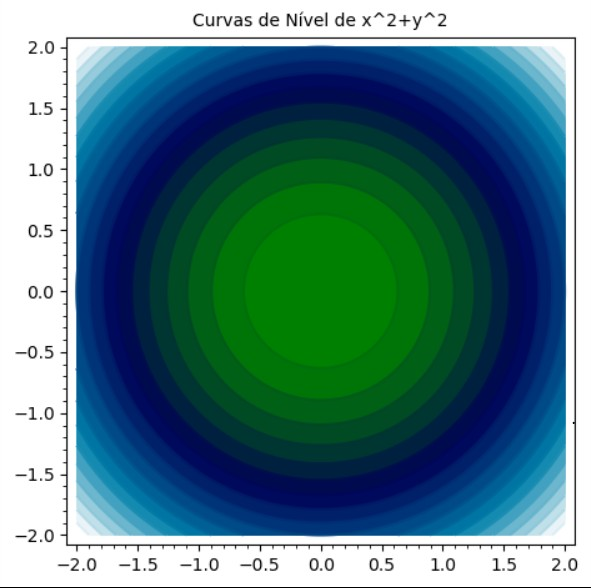
\includegraphics[width=\textwidth]{imagens/lista03/picture_lista03_q01_item01_02.jpg}
					\captionof{figure}{questão 1, item a), curvas de nível}
				\end{minipage}
			\end{center}
			
			\begin{center}
				% Primeira imagem
				\begin{minipage}{0.45\textwidth}
					\centering
					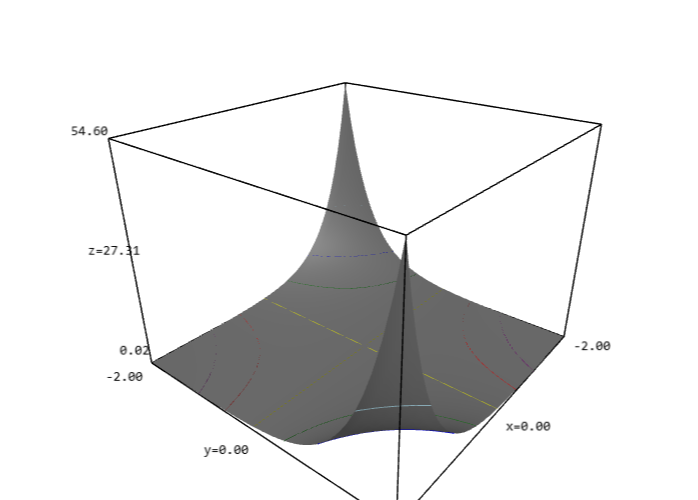
\includegraphics[width=\textwidth]{imagens/lista03/picture_lista03_q01_item02.png}
					\captionof{figure}{questão 1, item b), superfície}
				\end{minipage}
				\hfill
				% Segunda imagem
				\begin{minipage}{0.45\textwidth}
					\centering
					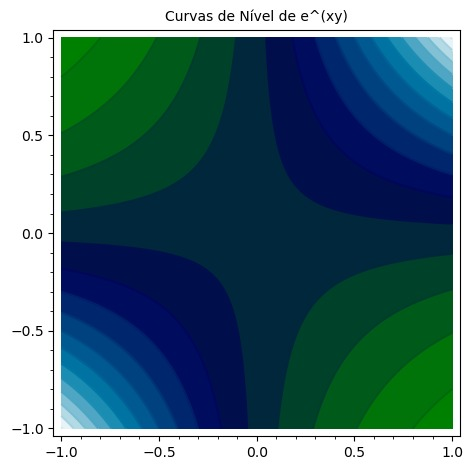
\includegraphics[width=\textwidth]{imagens/lista03/picture_lista03_q01_item02_02.jpg}
					\captionof{figure}{questão 1, item b), curvas de nível}
				\end{minipage}
			\end{center}
			
			\begin{center}
				% Primeira imagem
				\begin{minipage}{0.45\textwidth}
					\centering
					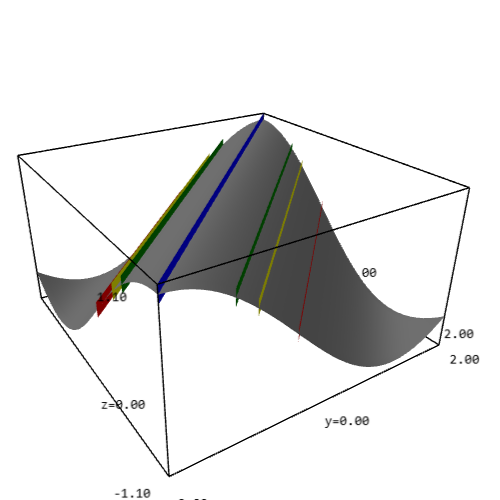
\includegraphics[width=\textwidth]{imagens/lista03/picture_lista03_q01_item03.png}
					\captionof{figure}{questão 1, item c), superfície}
				\end{minipage}
				\hfill
				% Segunda imagem
				\begin{minipage}{0.45\textwidth}
					\centering
					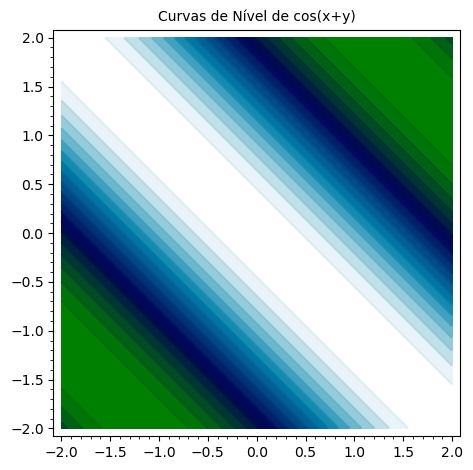
\includegraphics[width=\textwidth]{imagens/lista03/picture_lista03_q01_item03_02.jpg}
					\captionof{figure}{questão 1, item c), curvas de nível}
				\end{minipage}
			\end{center}
			
			Já nos itens d), e) e f), temos
			\begin{enumerate}[label=\alph*)]
				\item $f(x,y,z)=x+y+z$
				\item $f(x,y,z)=x^2+2y^2+3z^2$
				\item $f(x,y,z)=\sin(x^2+y^2+z^2)$
			\end{enumerate}
			
			Sendo todos campos escalares do tipo $f:S\subset \mathbb{R}^^3\rightarrow \mathbb{R}$, podemos representar as curvas de nível, por meio de superfícies no espaço. Nas figuras 7, 8 e 9 temos as imagens plotadas.
			
			\begin{center}
				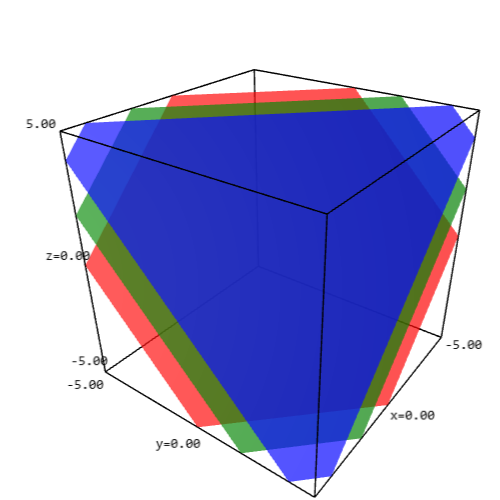
\includegraphics[width=0.3\textwidth]{imagens/lista03/picture_lista03_q01_item04.png}
				\captionof{figure}{questão 1, item d)}
			\end{center}
			
			\begin{center}
				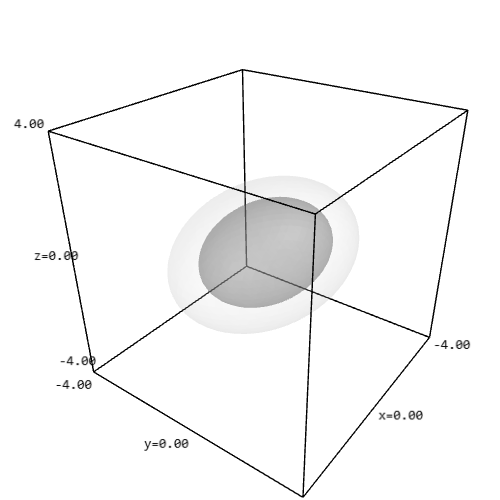
\includegraphics[width=0.3\textwidth]{imagens/lista03/picture_lista03_q01_item05.png}
				\captionof{figure}{questão 1, item e)}
			\end{center}
			
			\begin{center}
				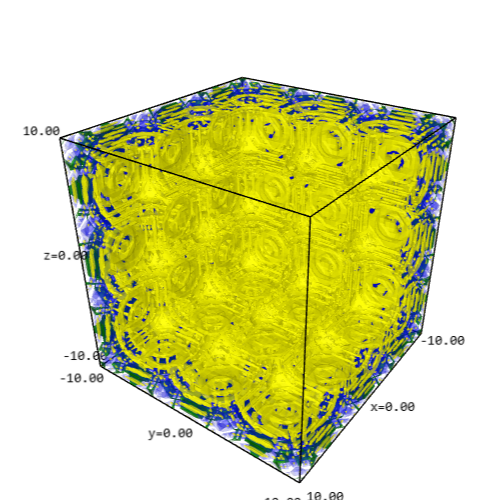
\includegraphics[width=0.3\textwidth]{imagens/lista03/picture_lista03_q01_item06.png}
				\captionof{figure}{questão 1, item f)}
			\end{center}
			
			\begin{lstlisting}[style=python_estiloso, caption={estrutura do codigo da questão 1, itens a), b), c)}]
				# Definindo as variaveis
				var("x y z")
				
				# Plotando as superficies de nivel para f(x, y, z) = k
				# Cada k representa uma superficie no espaco 3D
				superficie_1 = implicit_plot3d('equacao' == valor1,
				(x, -5, 5), (y, -5, 5), (z, -5, 5), color='red', opacity=0.7)
				superficie_2 = implicit_plot3d('equacao' == valor2,
				(x, -5, 5), (y, -5, 5), (z, -5, 5), color='green', opacity=0.7)
				superficie_3 = implicit_plot3d('equacao' == valor3,
				(x, -5, 5), (y, -5, 5), (z, -5, 5), color='blue', opacity=0.7)
				
				# Combinando e exibindo as superficies em um unico grafico
				(superficie_1 + superficie_2 + superficie_3).show(aspect_ratio=1,
				title='Superficies de Nivel para f(x,y,z)='equacao')
			\end{lstlisting}
			
		\end{solucao}
		
		\begin{exercicio}{2}
			Desenhe em ambiente computacional as seguintes figuras, marque um ponto sobre elas e trace uma curva sobre a sua superfície.
			\begin{itemize}
				\item Parabolóide elíptico: $S = \{(x, y, z) \in \mathbb{R}^3 \mid z = \tfrac{x^2}{a^2} + \tfrac{y^2}{b^2} \}$
				\item Parabolóide hiperbólico: $S = \{(x, y, z) \in \mathbb{R}^3 \mid z = \tfrac{x^2}{a^2} - \tfrac{y^2}{b^2} \}$
			\end{itemize}
			Escolha a sua descrição preferida para as superfícies (campos vetoriais), implícita ou paramétrica e justifique a sua preferência.
		\end{exercicio}
		
		\begin{solucao}
			Para essa questão, foram escolhidos $a=2$ e $b=3$. Nas figuras 10 e 11 estão as plotagens dos gráficos.
			
			Para plotar as superfícies em questão, o mais simples é utilizar a plotagem implícita, pois o enunciado dá o valor de $z$ em função de $x$ e $y$. Assim, utilizando a função "plot3d", o parabolóide elíptico pode ser descrito por $\big(x,y,\tfrac{x^2}{4}+\tfrac{y^2}{9}\big)$, e o parabolóide hiperbólico pode ser descrito por $\big(x,y,\tfrac{x^2}{4}-\tfrac{y^2}{9}\big)$.
			
			Para plotar as curvas, no entanto, podemos atribuir valores arbitrários associados a um parâmetro $t$ a $x$, $y$ e, consequentemente, a $z$. Uma substituição conveniente seria $x=2t$ e $y=3t$, o que implicaria $z=2t$ e $z=0$, no parabolóide elíptico e hiperbólico, respectivamente. 
			
			
			\begin{center}
				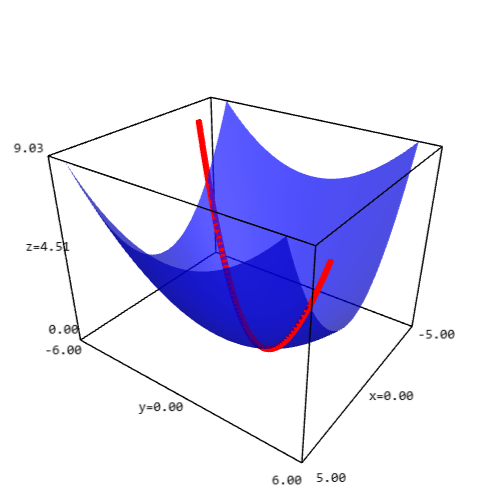
\includegraphics[width=0.3\textwidth]{imagens/lista03/picture_lista03_q02_item01.png}
				\captionof{figure}{questão 2, parabolóide elíptico}
			\end{center}
			
			\begin{center}
				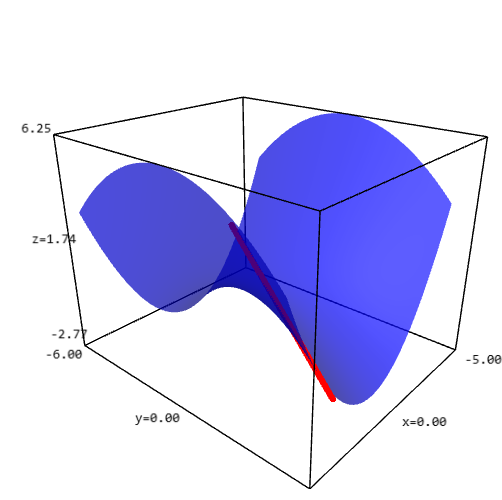
\includegraphics[width=0.3\textwidth]{imagens/lista03/picture_lista03_q02_item02.png}
				\captionof{figure}{questão 2, parabolóide hiperbólico}
			\end{center}
			
			\vspace{\baselineskip}
		\end{solucao}
		
		
		\begin{exercicio}{3}
			Desenhe duas ou mais opções de superfícies de rotação que te pareçam interessantes. Superfícies de rotação emergem da rotação de uma curva geratriz em torno de um eixo. Considere uma curva plana contida no plano $\Pi_{xz}$ da forma $\alpha(u) = (f(u), 0, g(u))$, $u \in I \subset \mathbb{R}$ e produza a rotação em torno do eixo vertical variando o parametro $v$ da seguinte forma
			\[
			X(u, v) = (f(u) \cos{v}, f(u)\sin{v}, g(u))
			\]
			Produza uma animação da curva geratriz com a variação do parâmetro.
		\end{exercicio}
		
		\begin{solucao}
			As superfícies de rotação escolhidas foram:
			\begin{itemize}
				\item Esfera: $f(u)=\cos(u)$ e $g(u)=\sin(u)$
				\item Toro: $f(u)=\cos(u)+5$ e $g(u)=\sin(u)$
			\end{itemize}
			
			As figuras 12 e 13 apresentam uma das imagens geradas nessas animações.
			
			\begin{center}
				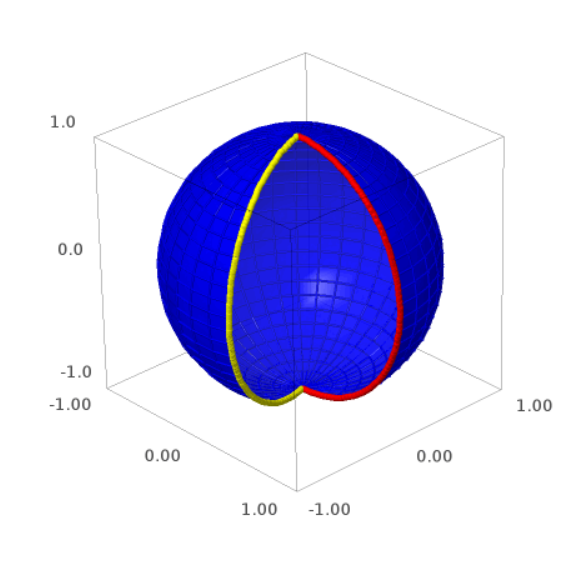
\includegraphics[width=0.3\textwidth]{imagens/lista03/picture_lista03_q03_item01.png}
				\captionof{figure}{questão 3, esfera}
			\end{center}
			
			\begin{center}
				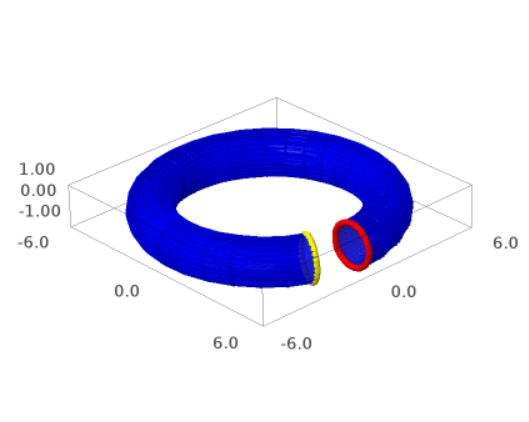
\includegraphics[width=0.3\textwidth]{imagens/lista03/picture_lista03_q03_item02.png}
				\captionof{figure}{questão 3, toro}
			\end{center}
			
			\vspace{\baselineskip}
		\end{solucao}
		
		\begin{exercicio}{4}
			Escolha um conceito de física para representar computacionalmente como campo vetorial.
		\end{exercicio}
		
		\begin{solucao}
			O conceito de física escolhido foi a gravidade, ou seja, foi representado um campo gravitacional. As plotagens estão nas figuras 14 e 15.
			
			\begin{center}
				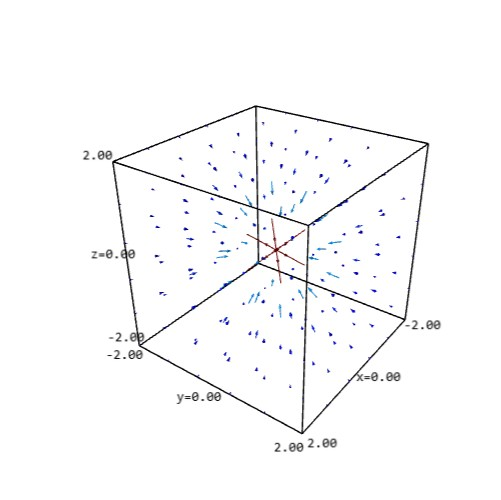
\includegraphics[width=0.3\textwidth]{imagens/lista03/picture_lista03_q04.jpg}
				\captionof{figure}{questão 4, campo gravitacional no espaço}
			\end{center}
			
			\begin{center}
				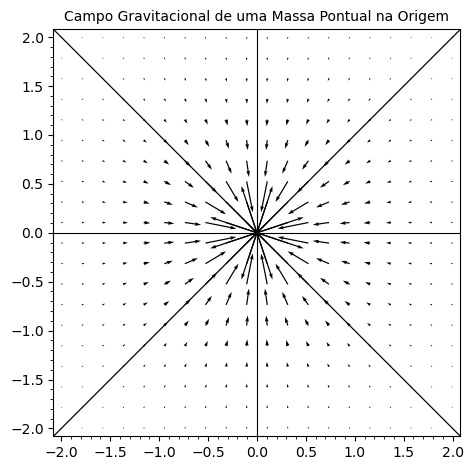
\includegraphics[width=0.3\textwidth]{imagens/lista03/picture_lista03_q04.png.jpg}
				\captionof{figure}{questão 3, campo gravitacional no plano}
			\end{center}
		\end{solucao}
		\subsection{Parte 2 (teórico)}
		\begin{exercicio}{1}
			(Apostol Calc II sec. 8.3 (pp 276) Exercício 2)
			Faça o esboço do conjunto e decida se é um conjunto aberto. O esboço pode ser feito tanto computacionalmente quanto à mão. A apresentação da demonstração é opcional.
		\end{exercicio}
		
		\begin{solucao}
			\begin{enumerate}[label=\alph*)]
				\item $\{(x,y) \mid x^2+y^2<1\}$ é um conjunto aberto.
				\begin{center}
					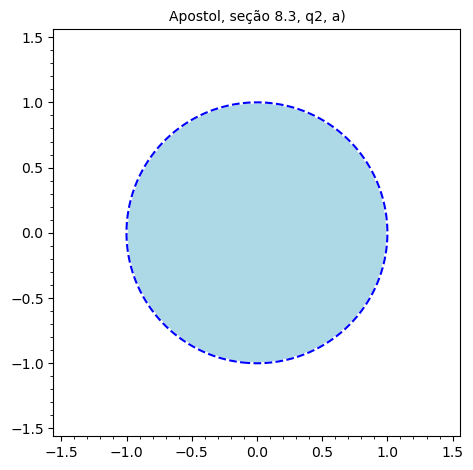
\includegraphics[width=0.25\textwidth]{imagens/lista03/picture_lista03.02_q01_item01.png}
					\captionof{figure}{$x^2+y^2<1$}
				\end{center}
				\item $\{(x,y) \mid 3x^2+2y^2<6\}$ é um conjunto aberto.
				\begin{center}
					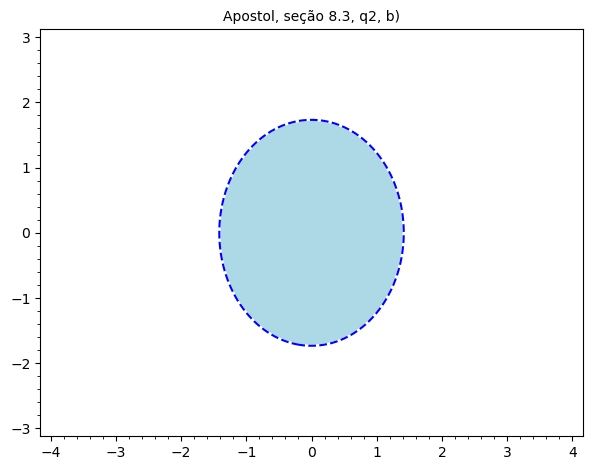
\includegraphics[width=0.25\textwidth]{imagens/lista03/picture_lista03.02_q01_item02.png}
					\captionof{figure}{$3x^2+2y^2<6$}
				\end{center}
				\item $\{(x,y) \mid |x|<1, |y|<1\}$ é um conjunto aberto.
				\begin{center}
					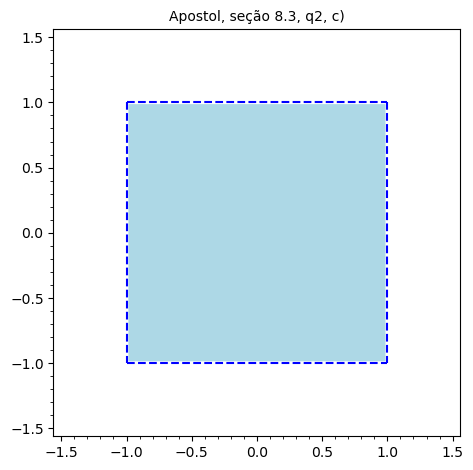
\includegraphics[width=0.25\textwidth]{imagens/lista03/picture_lista03.02_q01_item03.png}
					\captionof{figure}{$ |x|<1, |y|<1$}
				\end{center}
				\item $\{(x,y) \mid x\geq0, y>0\}$ não é um conjunto aberto.
				\begin{center}
					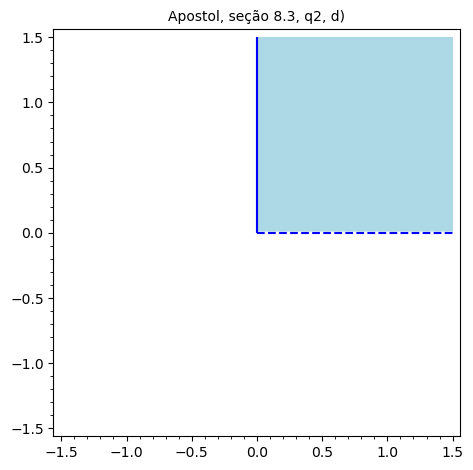
\includegraphics[width=0.25\textwidth]{imagens/lista03/picture_lista03.02_q01_item04.png}
					\captionof{figure}{$ x\geq0, y>0$}
				\end{center}
				\item $\{(x,y) \mid |x|\leq1, |y|\leq1\}$ não é um conjunto aberto.
				\begin{center}
					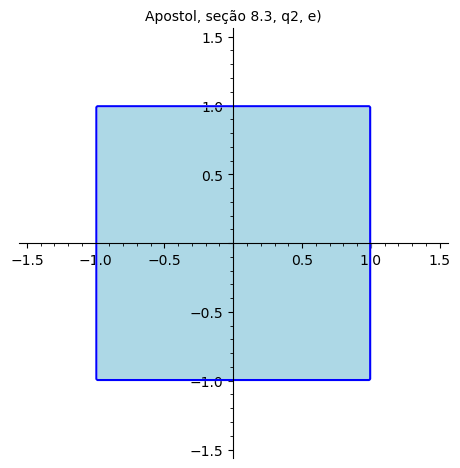
\includegraphics[width=0.25\textwidth]{imagens/lista03/picture_lista03.02_q01_item05.png}
					\captionof{figure}{$|x|\leq1, |y|\leq1$}
				\end{center}
				\item $\{(x,y) \mid x>0, y<0\}$ é um conjunto aberto.
				\begin{center}
					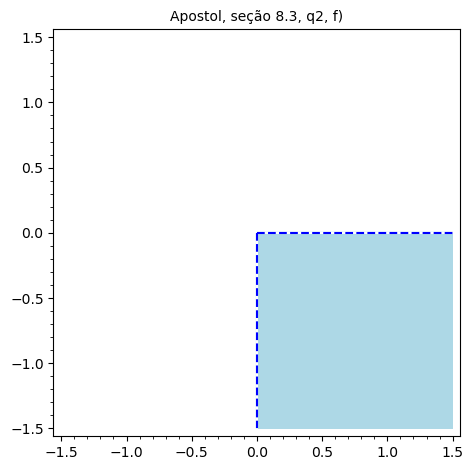
\includegraphics[width=0.25\textwidth]{imagens/lista03/picture_lista03.02_q01_item06.png}
					\captionof{figure}{$x>0, y<0$}
				\end{center}
				\item $\{(x,y) \mid xy<1\}$ é um conjunto aberto.
				\begin{center}
					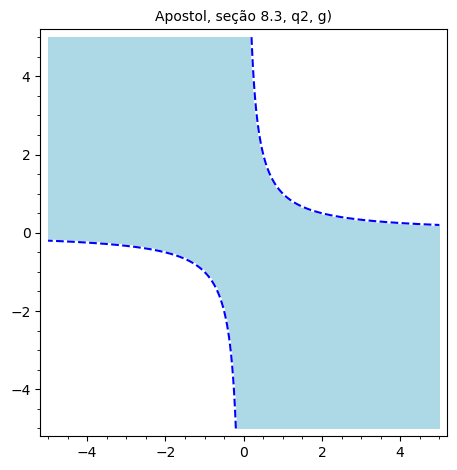
\includegraphics[width=0.25\textwidth]{imagens/lista03/picture_lista03.02_q01_item07.png}
					\captionof{figure}{$xy<1$}
				\end{center}
				\item $\{(x,y) \mid x\in [1,2], y\in (3,4)\}$ não é um conjunto aberto.
				\begin{center}
					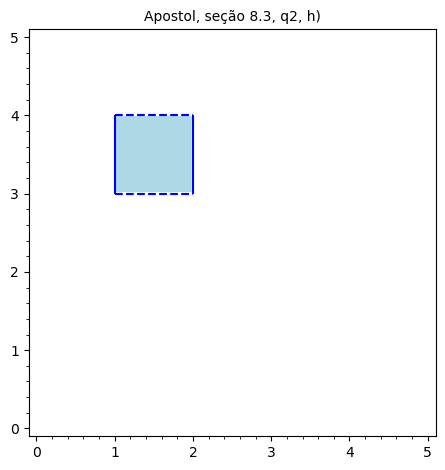
\includegraphics[width=0.25\textwidth]{imagens/lista03/picture_lista03.02_q01_item08.png}
					\captionof{figure}{$x\in [1,2], y\in (3,4)$}
				\end{center}
				\item $\{(x,y) \mid x\in (1,2), y>0\}$ é um conjunto aberto.
				\begin{center}
					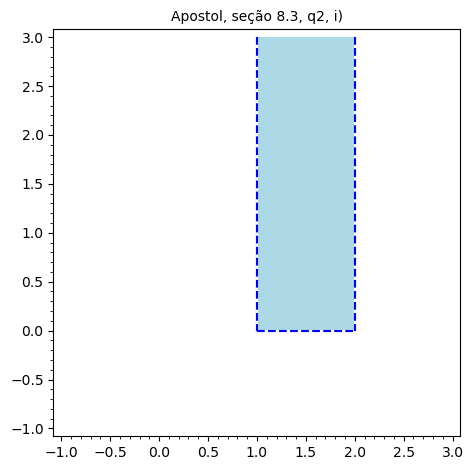
\includegraphics[width=0.25\textwidth]{imagens/lista03/picture_lista03.02_q01_item09.png}
					\captionof{figure}{$x\in (1,2), y>0$}
				\end{center}
				\item $\{(x,y) \mid x\geq y\}$ não é um conjunto aberto.
				\begin{center}
				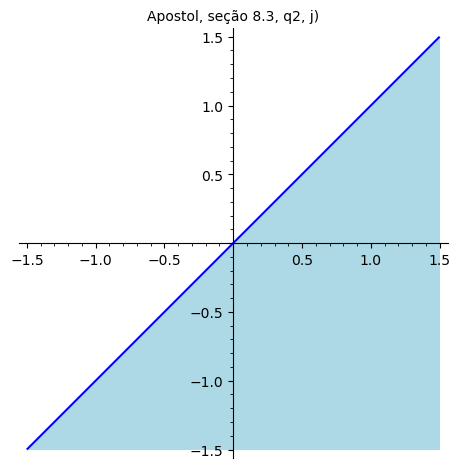
\includegraphics[width=0.25\textwidth]{imagens/lista03/picture_lista03.02_q01_item10.png}
				\captionof{figure}{$x\geq y$}
				\end{center}
				\item $\{(x,y) \mid x> y\}$ é um conjunto aberto.
				\begin{center}
				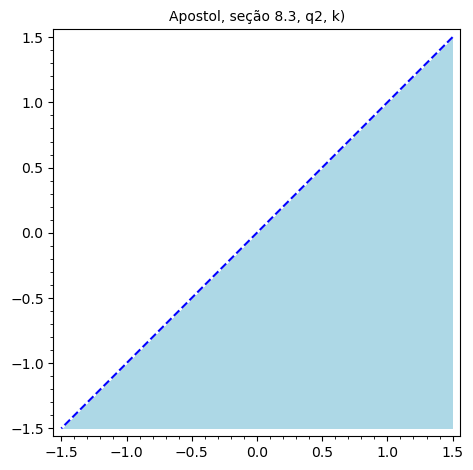
\includegraphics[width=0.25\textwidth]{imagens/lista03/picture_lista03.02_q01_item11.png}
				\captionof{figure}{$x> y$}
				\end{center}
				\item $\{(x,y) \mid y>x^2, |x|<2\}$ é um conjunto aberto.
				\begin{center}
				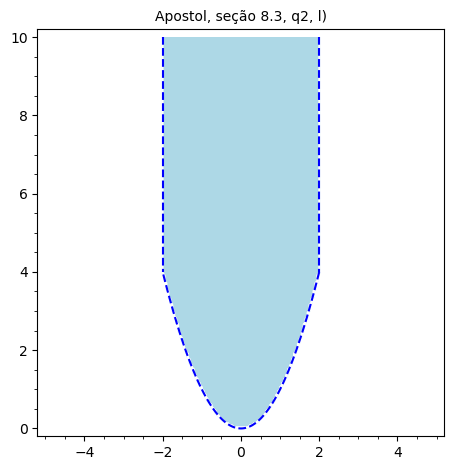
\includegraphics[width=0.25\textwidth]{imagens/lista03/picture_lista03.02_q01_item12.png}
				\captionof{figure}{$y>x^2, |x|<2$}
				\end{center}
				\item $\{(x,y) \mid (x^2+y^2-1)(4-x^2-y^2)>0\}$ é um conjunto aberto.
				\begin{center}
				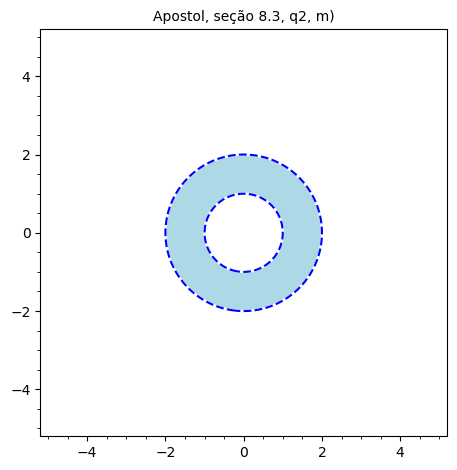
\includegraphics[width=0.25\textwidth]{imagens/lista03/picture_lista03.02_q01_item13.png}
				\captionof{figure}{$(x^2+y^2-1)(4-x^2-y^2)>0$}
				\end{center}
				\item $\{(x,y) \mid (2x-x^2-y^2)(x^2+y^2-x)>0\}$ é um conjunto aberto.
				\begin{center}
				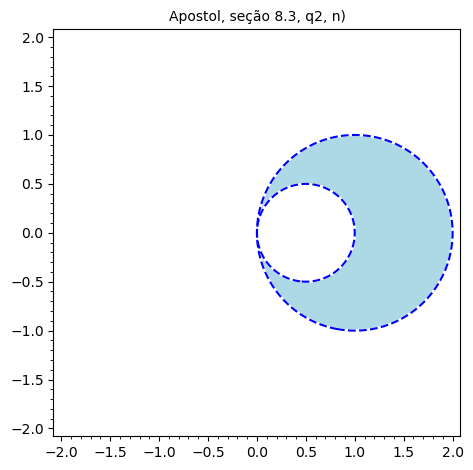
\includegraphics[width=0.25\textwidth]{imagens/lista03/picture_lista03.02_q01_item14.png}
				\captionof{figure}{$(2x-x^2-y^2)(x^2+y^2-x)>0$}
				\end{center}
			\end{enumerate}
		\end{solucao}
		
		\begin{exercicio}{2}
			(Apostol Calc II sec. 8.3 (pp 276) Exercício 3).
			Faça o esboço do conjunto e decida se é um conjunto aberto. O esboço pode ser feito tanto computacionalmente quanto à mão. A apresentação da demonstração é opcional.
		\end{exercicio}
		
		\begin{solucao}
			\begin{enumerate}[label=\alph*)]
				\item $\{(x,y,z) \mid z^2-x^2-y^2-1>0\}$ é um conjunto aberto.
				\begin{center}
					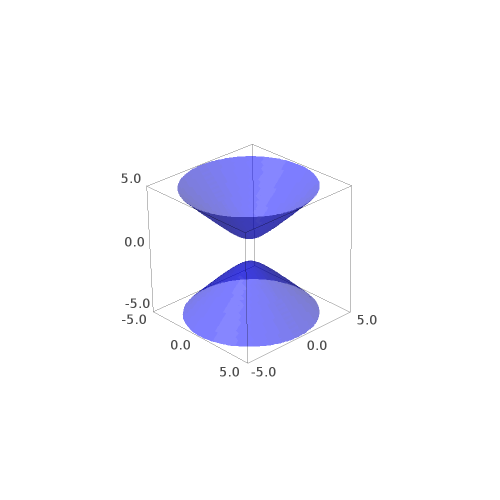
\includegraphics[width=0.25\textwidth]{imagens/lista03/picture_lista03.02_q02_item01.png}
					\captionof{figure}{$z^2-x^2-y^2-1>0$}
				\end{center}
				\item $\{(x,y,z) \mid |x|<1, |y|<1, |z|<1\}$ é um conjunto aberto.
				\begin{center}
					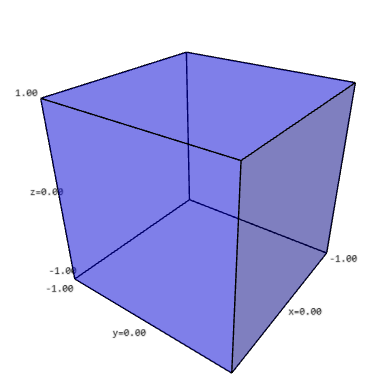
\includegraphics[width=0.25\textwidth]{imagens/lista03/picture_lista03.02_q02_item02.png}
					\captionof{figure}{$|x|<1, |y|<1, |z|<1$}
				\end{center}
				\item $\{(x,y,z) \mid x+y+z<1\}$ é um conjunto aberto.
				\begin{center}
					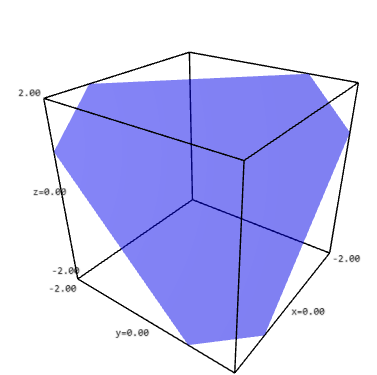
\includegraphics[width=0.25\textwidth]{imagens/lista03/picture_lista03.02_q02_item03.png}
					\captionof{figure}{$x+y+z<1$}
				\end{center}
				\item $\{(x,y) \mid |x|\leq1, |y|<1, |z|<1\}$ não é um conjunto aberto.
				\begin{center}
					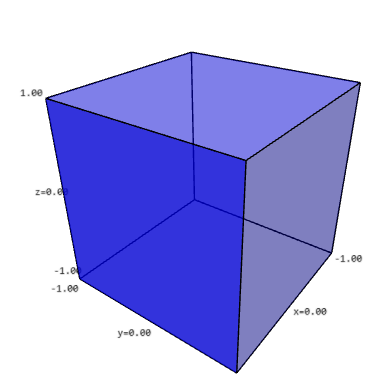
\includegraphics[width=0.25\textwidth]{imagens/lista03/picture_lista03.02_q02_item04.png}
					\captionof{figure}{$|x|\leq1, |y|<1, |z|<1$}
				\end{center}
				\item $\{(x,y) \mid x+y+z<1, x>0, y>0, z>0\}$ é um conjunto aberto.
				\begin{center}
					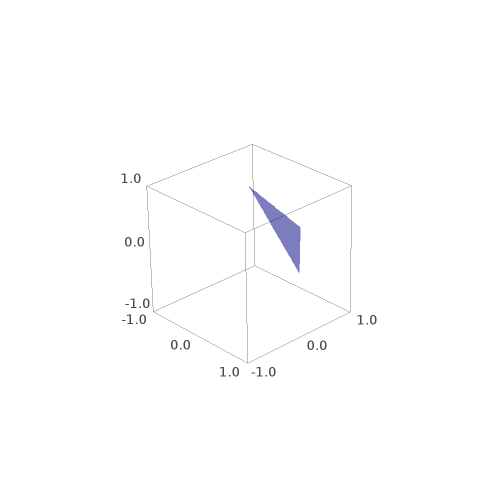
\includegraphics[width=0.25\textwidth]{imagens/lista03/picture_lista03.02_q02_item05.png}
					\captionof{figure}{$x+y+z<1, x>0, y>0, z>0$}
				\end{center}
				\item $\{(x,y) \mid x^2+4y^2+4z^2-2x+16y+40z+113>0\}$ é um conjunto aberto.
				\begin{center}
					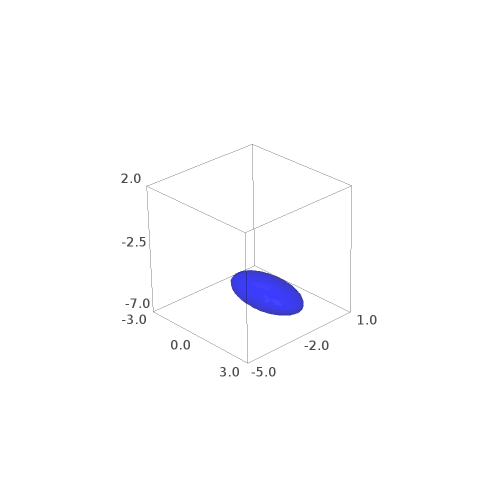
\includegraphics[width=0.25\textwidth]{imagens/lista03/picture_lista03.02_q02_item06.png}
					\captionof{figure}{$x^2+4y^2+4z^2-2x+16y+40z+113>0$}
				\end{center}
			\end{enumerate}
		\end{solucao}
		
		\begin{exercicio}{3}
			(Apostol Calc II sec. 8.3 (pp 277) Exercício 6). Faça o esboço do
			conjunto e decida se é um conjunto aberto. O esboço pode ser feito tanto computacionalmente
			quanto à mão. Justifique o seu raciocínio.
		\end{exercicio}
		
		\begin{solucao}
			\begin{enumerate}[label=\alph*)]
				\item $\{(x,y) \mid x^2+y^2\geq0\}$ é um conjunto tanto aberto e quanto fechado (o próprio $\mathbb{R}^2$).
				\begin{center}
					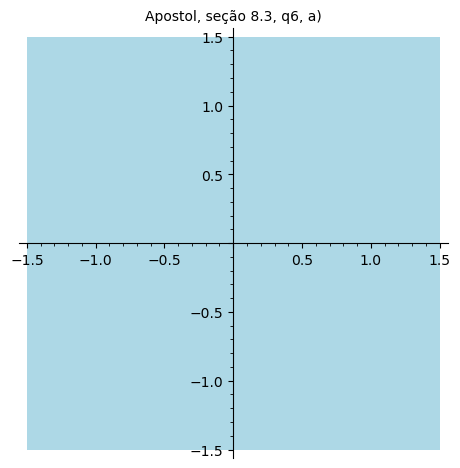
\includegraphics[width=0.25\textwidth]{imagens/lista03/picture_lista03.02_q03_item01.png}
					\captionof{figure}{$x^2+y^2\geq 0$}
				\end{center}
				\item $\{(x,y) \mid x^2+y^2< 0\}$ é um conjunto tanto aberto quanto fechado (vazio).
				\begin{center}
					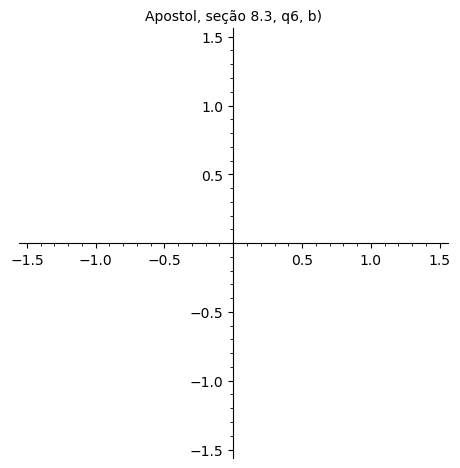
\includegraphics[width=0.25\textwidth]{imagens/lista03/picture_lista03.02_q03_item02.png}
					\captionof{figure}{$x^2+y^2<0$}
				\end{center}
				\item $\{(x,y) \mid x^2+y^2\leq 1\}$ é um conjunto fechado apenas.
				\begin{center}
					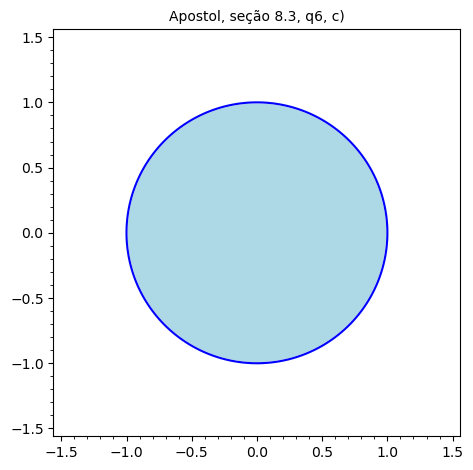
\includegraphics[width=0.25\textwidth]{imagens/lista03/picture_lista03.02_q03_item03.png}
					\captionof{figure}{$x^2+y^2\leq 1$}
				\end{center}
				\item $\{(x,y) \mid 1<x^2+y^2<2\}$ é um conjunto aberto apenas.
				\begin{center}
					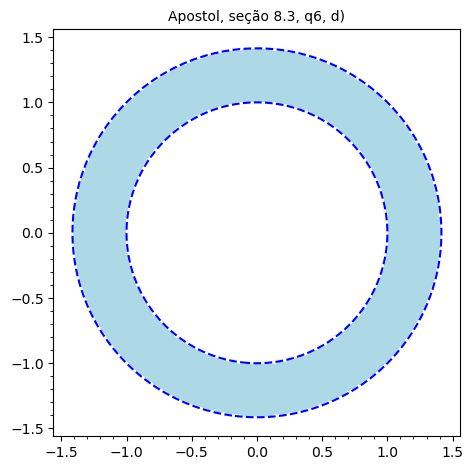
\includegraphics[width=0.25\textwidth]{imagens/lista03/picture_lista03.02_q03_item04.png}
					\captionof{figure}{$ 1<x^2+y^2<2$}
				\end{center}
				\item $\{(x,y) \mid 1\leq x^2+y^2\leq2\}$ é um conjunto fechado apenas.
				\begin{center}
					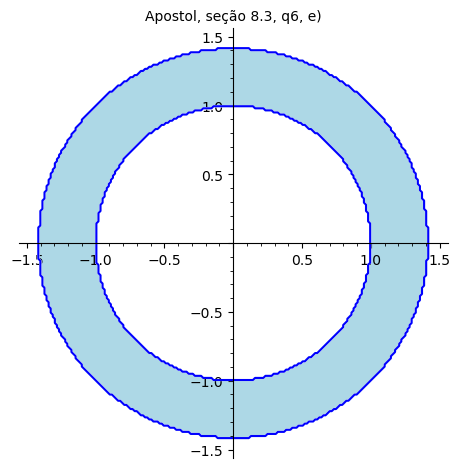
\includegraphics[width=0.25\textwidth]{imagens/lista03/picture_lista03.02_q03_item05.png}
					\captionof{figure}{$1\leq x^2+y^2\leq2$}
				\end{center}
				\item $\{(x,y) \mid 1< x^2+y^2\leq2\}$ não é um conjunto aberto, nem fechado.
				\begin{center}
					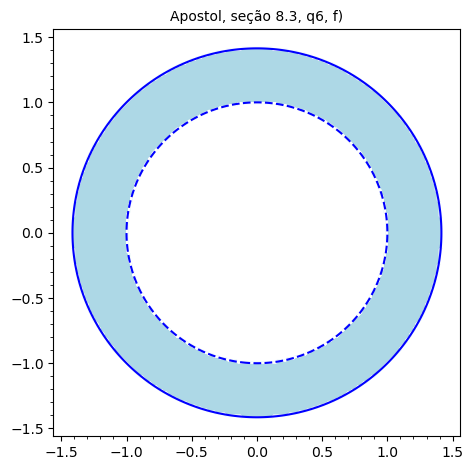
\includegraphics[width=0.25\textwidth]{imagens/lista03/picture_lista03.02_q03_item06.png}
					\captionof{figure}{$1< x^2+y^2\leq2$}
				\end{center}
				\item $\{(x,y) \mid x\in [1,2], y\in [3,4]\}$ é um conjunto fechado apenas.
				\begin{center}
					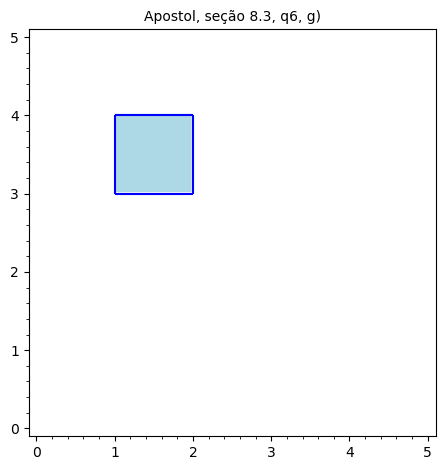
\includegraphics[width=0.25\textwidth]{imagens/lista03/picture_lista03.02_q03_item07.png}
					\captionof{figure}{$x\in [1,2], y\in [3,4]$}
				\end{center}
				\item $\{(x,y) \mid x\in [1,2], y\in [3,4)\}$ não é um conjunto aberto, nem fechado.
				\begin{center}
					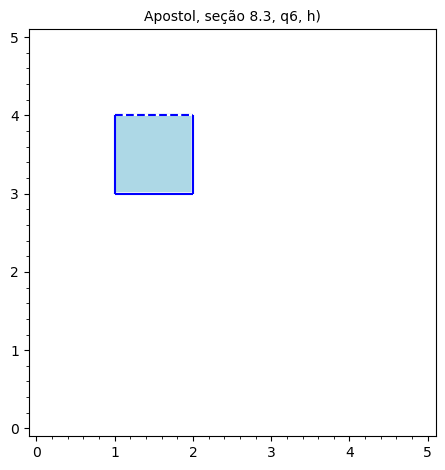
\includegraphics[width=0.25\textwidth]{imagens/lista03/picture_lista03.02_q03_item08.png}
					\captionof{figure}{$x\in [1,2], y\in [3,4)$}
				\end{center}
				\item $\{(x,y) \mid x^2=y\}$ é um conjunto fechado apenas.
				\begin{center}
					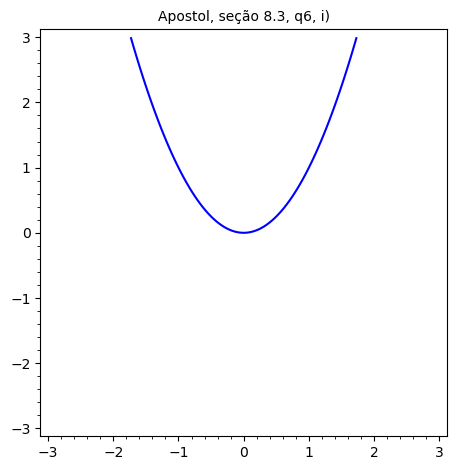
\includegraphics[width=0.25\textwidth]{imagens/lista03/picture_lista03.02_q03_item09.png}
					\captionof{figure}{$x^2=y$}
				\end{center}
				\item $\{(x,y) \mid x^2\leq y\}$ é um conjunto fechado apenas.
				\begin{center}
					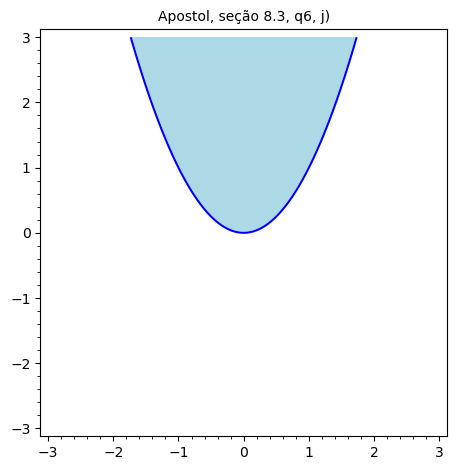
\includegraphics[width=0.25\textwidth]{imagens/lista03/picture_lista03.02_q03_item10.png}
					\captionof{figure}{$x^2\leq y$}
				\end{center}
				\item $\{(x,y) \mid x^2\leq y, |x|<2\}$ não é um conjunto aberto, nem fechado.
				\begin{center}
					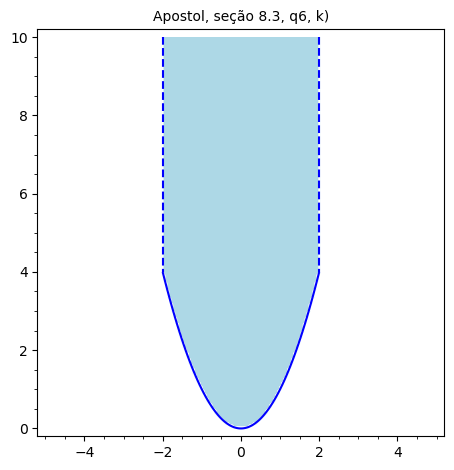
\includegraphics[width=0.25\textwidth]{imagens/lista03/picture_lista03.02_q03_item11.png}
					\captionof{figure}{$x^2\leq y, |x|<2$}
				\end{center}
				\item $\{(x,y) \mid x^2\leq y, |x|\leq 2\}$ é um conjunto fechado apenas.
				\begin{center}
					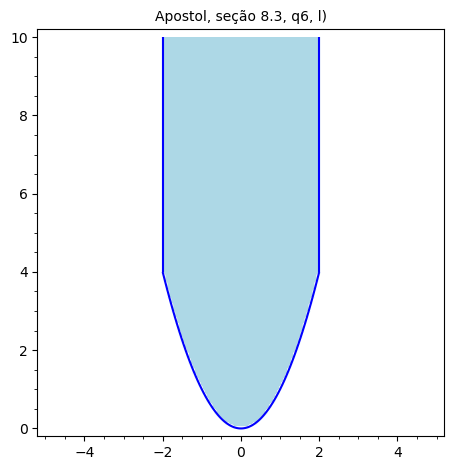
\includegraphics[width=0.25\textwidth]{imagens/lista03/picture_lista03.02_q03_item12.png}
					\captionof{figure}{$x^2\leq y, |x|\leq 2$}
				\end{center}
			\end{enumerate}
		\end{solucao}
		
		\begin{exercicio}{7}
			O conjunto $\{\tfrac{1}{n} \mid n \in \mathbb{N}-\{0\}\} \subset \mathbb{R}$ é aberto? É fechado?
		\end{exercicio}
		
		\begin{solucao}
			\begin{definicao}[Conjunto aberto]
				O conjunto $U\subset \mathbb{R}^{n}$ é dito aberto quando $\forall p\in U$, $\exists r>0\mid B(p,r)\subset U$, isto é, todo ponto $p\in U$ é ponto interior, isto é, $U=int(U)$
			\end{definicao}
			
			Suponha que $A=\{\tfrac{1}{n} \mid n \in \mathbb{N}-\{0\}\}$ é aberto e tome $\tfrac{1}{k}$ arbitrário de $A$. Como $A$ é aberto,
			
			\[
			\exists r>0\mid B(\tfrac{1}{k}, r)\subset A
			\]
			\[
			\exists r>0\mid x\in B(\tfrac{1}{k}, r) \Rightarrow x\in A
			\]
			
			No entanto, note que na bola $B(\tfrac{1}{k}, r)$ existem infinitos números irracionais. Como o conjunto $A$ é formado apenas por números racionais, temos que $\forall r>0$, $\exists x>0\mid x\in B(\tfrac{1}{k},r)$ e $x\notin A$.
			
			Logo, temos uma contradição com a suposição de que $A$ é aberto. Portanto, $A$ não é aberto.
			
			\begin{definicao}[Conjunto fechado]
				Um subconjunto $S$ de $\mathbb{R}^n$ é dito fechado quando o seu complementar $\mathbb{R}^{n}-S$ é aberto.
			\end{definicao}
			
			Suponha que $A=\{\tfrac{1}{n} \mid n \in \mathbb{N}-\{0\}\}$ é fechado. Logo, $A^C$ é aberto. Em particular, como $0\in A^C$, temos
			
			\[
			\exists r>0\mid B(0,r)\subset A
			\]
			\[
			\exists r>0\mid x<r\Rightarrow x\in A
			\]
			
			No entanto, note que no intervalo $(0,r)$ existem infinitos números irracionais. Como o conjunto $A$ é formado apenas por números racionais, temos que $\forall r>0$, $\exists x>0\mid x<r$ e $x\notin A$.
			
			Logo, temos uma contradição com a suposição de que $A$ é fechado. Portanto, $A$ não é fechado.
		\end{solucao}
		
		\begin{exercicio}{9}
			Prove que
			\[
			\{(x, y)\in \mathbb{R}^2\mid y > 0\}
			\]
			é aberto.
		\end{exercicio}
		
		\begin{solucao}
			Tome um $(a,b)\in U=\{(x, y)\in \mathbb{R}^2\mid y > 0\}$ arbitrário. Queremos mostrar que $\exists r>0\mid B((a,b),r)\subset U$.
			
			Assim, como $b>0$, tome $r=b$. Seja $(c,d)\in B((a,b),b)$ outro ponto arbitrário.
			
			\[
			(c,d)\in B((a,b),b)\Rightarrow \|(c,d)-(a,b)\|<b
			\]
			\[
			\Rightarrow (c-a)^2+(d-b)^2<b^2 \Rightarrow (c-a)^2<b^2-(d-b)^2=d(2b-d)
			\]
			\[
			\Rightarrow 0<=(c-a)^2<d(2b-d)\Rightarrow 0<d(2b-d)
			\]
			
			Caso $d=0$, temos $0<0$ (absurdo).
			
			Caso $d<0$, temos $d<0$ e $2b-d>0 \Rightarrow d(2b-d)<0$ (absurdo).
			
			Logo, pela lei da tricotomia, $d>0\Rightarrow (c,d)\in U$.
			
			Portanto, $(c,d)\in B((a,b),b)\Rightarrow (c,d)\in U$.
			
			$\therefore B((a,b),b)\subset U \Rightarrow U$ é aberto. 
		\end{solucao}
	
\end{document}
